\chapter{Matching and Assignment Problem}

Hearing footsteps behind them, Ajur and Jura turned back and saw Rishnak, rushing to catch up with them and continue their discussion. Rishank wasted no time and started with saying that the edges analog of maximal independent set (set of non-adjacent vertices) is a maximal matching. Maximal matching is a set of edges that do not share any common end vertices. Rishnak showed a graph Figure \ref{16g1} and the maximal matching edges are colored red.
\begin{figure}
\begin{center}

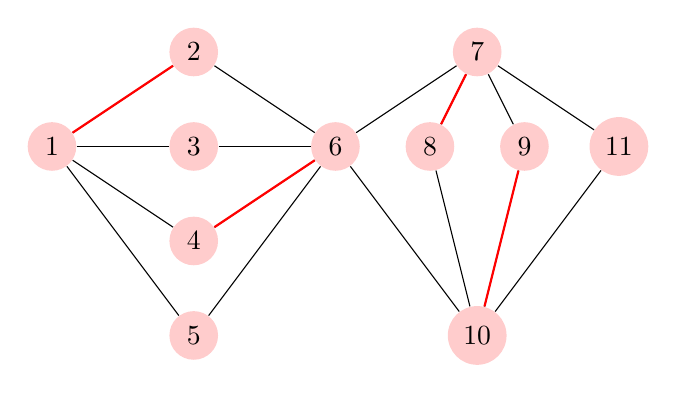
\begin{tikzpicture}
  [scale=.6,auto=left,every node/.style={circle,fill=red!20}]
  \node (n1) at (-1,1) {1};
  \node (n2) at (2,3)  {2};
  \node (n3) at (2,1)  {3};
  \node (n4) at (2,-1) {4};
  \node (n5) at (2, -3) {5};
  \node (n6) at (5,1)  {6};
  \node (n7) at (8,3)  {7};
  \node (n8) at (7,1) {8};
  \node (n9) at (9,1)  {9};
  \node (n10) at (8,-3)  {10};
  \node (n11) at (11,1) {11};

  \foreach \from/\to in {n1/n2,n1/n3,n1/n4,n1/n5,n2/n6,n3/n6/n4,n4/n6,n5/n6,n6/n7,n6/n10,n7/n8,n7/n9,n7/n11,
  n8/n10,n9/n10,n10/n11}
    \draw (\from) -- (\to);
\draw[-,thick,red]
  (n1) to (n2);
  \draw[-,thick,red]
  (n4) to (n6);
  \draw[-,thick,red]
  (n7) to (n8);
  \draw[-,thick,red]
  (n9) to (n10);
  \end{tikzpicture}
\caption{Maximal Matching edges in this graph are colored red}\label{16g1}
\end{center}
\end{figure}

Since this is a maximal matching - every edge is incident at one of the end vertices of the edges in the Maximal set. Hence the vertices $\{1,2,4,6,7,8,9,10\}$ form a vertex cover. However the minimum vertex cover is $\{1,6,7,10\}$. If we find a Maximal matching we know the bound on the size of the minimum vertex cover!.


A perfect matching is a matching such that all the vertices are the end vertices of the edges in the matching. For example Figure \ref{16g1} does not have a perfect matching.  But consider the following graph Figure \ref{16g2}; this graph has a maximal matching and all the vertices are present as one of the end vertices of the edges in the maximal matching.

\begin{figure}
\begin{center}
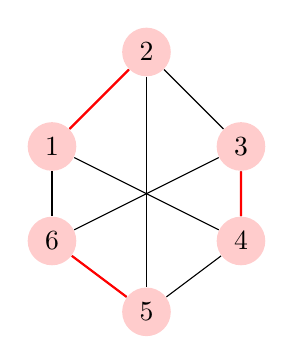
\begin{tikzpicture}
  [scale=.3,auto=left,every node/.style={circle,fill=red!20}]
  \node (n1) at (1,7) {1};
  \node (n2) at (5,11)  {2};
  \node (n3) at (9,7)  {3};
  \node (n4) at (9,3) {4};
  \node (n5) at (5,0)  {5};
  \node (n6) at (1,3) {6};
  
   \foreach \from/\to in {n1/n2,n2/n3,n3/n4,n4/n5,n5/n6,n1/n6,
  n2/n5, n6/n3,n1/n4}
    \draw (\from) -- (\to);
     \foreach \from/\to in {n1/n2,n5/n6,n3/n4}
    \draw[thick,red] (\from) -- (\to);
    \end{tikzpicture}
\caption{ This graph has a perfect matching and the edges in the perfect matching are marked red}\label{16g2}
\end{center}
\end{figure}
Rishnak then mentioned some interesting tidbits about Matching Problem.
A problem related to Matching got the Nobel prize in Economics in 2012 for Prof. Llyod Shapely and 
Prof. Alvin Roth.  Prof. David Gale and Prof. Shapely introduced a problem called Stable Marriage Problem (which we will describe next) and Prof. Alvin Roth applied this for variety of applications including medical resident assignment problem, kidney transplants, etc.

Stable Marriage Problem may be stated as follows:
Given $n$ males and $n$ females and a list of preferences for each male and female, find a stable marriage for the whole group.
A marriage is unstable if there are a male and female who are not married to each other but prefer each other to their respective spouses. Otherwise, the marriage is stable.
Consider the preferences for males \ref{16t1} and females\ref{16t2} as follows:
\begin{table}
\begin{center}
\begin{tabular}{ |p{3cm}||p{1.5cm}||p{1.5cm} || p{1.5cm}|| }
 \hline
 \hline
 Male Name & First&Second&Third\\
 \hline
 Al  & Carla    &Ada&Bea\\
Bob&Ada&Bea&Carla\\
Caleb&Ada&Carla&Bea\\
 
 
 \hline
\end{tabular}
\caption{Male Preferences}\label{16t1}
\end{center}
\end{table}
\begin{table}
\begin{center}
\begin{tabular}{ |p{3cm}||p{1.5cm}||p{1.5cm} || p{1.5cm}|| }
 \hline
 \hline
 Female Name & First&Second&Third\\
 \hline
 Ada  & Al    &Bob&Caleb\\
Bea&Caleb&Al&Bob\\
Carla&Al&Caleb&Bob\\
 
 
 \hline
\end{tabular}
\caption{Female Preferences}\label{16t2}
\end{center}
\end{table}

For this preferences the following marriage is stable (Al, Carla), (Bob, Ada) and (Caleb, Bea) as there are no unstable pairs.
However, (Al, Carla), (Bob, Bea) and (Caleb, Ada) is unstable marriage as Bob prefers Ada than Bea and Ada prefers Bob to Caleb.
Gale and Shapely showed that there is always a stable marriage pair for any preferences and they provided an elegant algorithm.

\begin{enumerate}
    \item In the first round, each male proposes to the female he prefers most.
    \item Each female replies "maybe" to her suitor she most prefers and "no" to all other suitors. She is temporarily "engaged" to the male she most prefers so far. 
    \item In subsequent round, each unengaged male proposes to the most-preferred female\footnote{Each male starts from his most preferred female to the least preferred} to whom he has not yet proposed (regardless of whether the female is already engaged).
    \item Each female replies "maybe" if she is currently not engaged or if she prefers this male over her current provisional partner\footnote{Based on her preferences} (in this case, she rejects her current provisional partner who becomes unengaged). The provisional nature of engagements preserves the right of an already-engaged female to "trade up" (and, in the process, to "jilt" her until-then partner).
   \item Repeat steps 3 and 4 until everyone is engaged
\end{enumerate}

Applying this procedure to example \ref{16t1} and \ref{16t2}, after the first round, Al is temporarily engaged to Carla and Bob is temporarily engaged to Ada (Both Bob and Caleb opts for Ada - but Ada prefers Bob to Caleb). Next round Caleb goes to Carla (who is temporarily engaged to Al). Since Carla prefers Al to Caleb, Caleb's offer is rejected. Now Caleb goes to Bea (as his last choice) and Bea takes Caleb as she did not have a suitor so far. So the algorithm terminates with the stable marriage pair of (Al, Carla), (Bob, Ada) and (Caleb, Bea). 

Ajur said this algorithm sounded like like a musical chair assignment where males are searching for the females!

Rishnak said that another application of a Matching problem is an Optimal Assignment Problem. 
Problem statement: Assign jobs to a group of workers and cost of each worker doing each job is give. Find an assignment of workers to jobs so as to minimize the total cost. This problem can be viewed as a bipartite graph with workers in one partition and jobs on the other partition. The edge from worker $i$ to job $j$ gives the cost of worker $i$ doing the job $j$.
We will assume that the number of workers is equal to the number of jobs ($n$).
\begin{table}
\begin{center}
\begin{tabular}{ ||p{2cm}||p{2cm}||p{1.5cm} ||p{1.5cm}|| }
 \hline
 
  & Salesmanr&Tutor&Chef\\
 \hline
 Al  & 17   &40&45\\
 Bob& 23&60&35\\
 Caleb&21&40&25\\

 
 \hline
\end{tabular}
\caption{Cost Matrix - Rows are workers and Columns are the jobs and Cost is given as a matirx }\label{16t3}
\end{center}
\end{table}

\begin{enumerate}
\item For each row of the matrix\footnote{matrix is a two dimensional array}, find the smallest element and subtract that from every element in its row.
\item Do step 1 for all columns.
\item Cover all zeros in the matrix using minimum number of horizontal  and vertical lines.
\item If the minimum number of covering lines is n, an optimal assignment is possible and we are done. Else  proceed to step 5.
\item Determine the smallest entry not covered by any line. Subtract this entry from each uncovered row, and then add it to each covered column. Return to step 3.
\end{enumerate}

At the end of the first step we get Table \ref{16t4}
\begin{table}
\begin{center}
  \begin{tikzpicture}
    \matrix (M)[matrix of math nodes,left delimiter={[},right delimiter={]}]{
     0&23&28\\
     0&37&12\\
     0&19&4\\
     };
     %\draw[thick,black](M-1-1.west)--(M-1-4.east);
     %\draw[thick,black](M-1-1.north)--(M-4-1.south);
     %\draw[thick,black](M-1-3.north)--(M-4-3.south);
  \end{tikzpicture}

\caption{At the end of first step }\label{16t4}
\end{center}
\end{table}
At the end of second step we get Table  \ref{16t5}
\begin{table}
\begin{center}
  \begin{tikzpicture}
    \matrix (M)[matrix of math nodes,left delimiter={[},right delimiter={]}]{
     0&4&24\\
     0&18&8\\
     0&0&0\\
     };
     %\draw[thick,black](M-1-1.west)--(M-1-4.east);
     %\draw[thick,black](M-1-1.north)--(M-4-1.south);
     %\draw[thick,black](M-1-3.north)--(M-4-3.south);
  \end{tikzpicture}

\caption{At the end of second step }\label{16t5}
\end{center}
\end{table}

Since two lines cover all the zeros as shown in  Table \ref{16t6}
\begin{table}
\begin{center}
  \begin{tikzpicture}
    \matrix (M)[matrix of math nodes,left delimiter={[},right delimiter={]}]{
     0&4&24\\
     0&18&8\\
     0&0&0\\
     };
     \draw[thick,black](M-3-1.west)--(M-3-3.east);
     \draw[thick,black](M-1-1.north)--(M-3-1.south);
     %\draw[thick,black](M-1-3.north)--(M-4-3.south);
  \end{tikzpicture}

\caption{Two lines cover all 0's}\label{16t6}
\end{center}
\end{table}

So we resort to step 5, taking the smallest entry among uncovered entries and do step 5 resulting in the following Tables \ref{16t7} and \ref{16t8} 
\begin{table}
\begin{center}
  \begin{tikzpicture}
    \matrix (M)[matrix of math nodes,left delimiter={[},right delimiter={]}]{
     -4&0&20\\
     -4&14&4\\
     0&0&0\\
     };
     \draw[thick,black](M-3-1.west)--(M-3-3.east);
     \draw[thick,black](M-1-1.north)--(M-3-1.south);
     %\draw[thick,black](M-1-3.north)--(M-4-3.south);
  \end{tikzpicture}

\caption{Subtracting 4 from uncovered rows}\label{16t7}
\end{center}
\end{table}
\begin{table}
\begin{center}
  \begin{tikzpicture}
    \matrix (M)[matrix of math nodes,left delimiter={[},right delimiter={]}]{
     0&0&20\\
     0&14&4\\
     4&0&0\\
     };
     \draw[thick,black](M-3-1.west)--(M-3-3.east);
     \draw[thick,black](M-1-1.north)--(M-3-1.south);
     %\draw[thick,black](M-1-3.north)--(M-3-3.south);
     %\draw[thick,black](M-1-1.north)--(M-3-1.south);
     %\draw[thick,black](M-1-2.north)--(M-3-2.south);
  \end{tikzpicture}

\caption{Adding 4 to covered columns }\label{16t8}
\end{center}
\end{table}

Now we have exactly three lines to cover all 0's as shown in Table \ref{16t9} and we are done. The assignment of Al to Tutor,
Bob to Salesman and Caleb to Chef with a total cost of 40+23+25=88. 
\begin{table}
\begin{center}
  \begin{tikzpicture}
    \matrix (M)[matrix of math nodes,left delimiter={[},right delimiter={]}]{
     0&0&20\\
     0&14&4\\
     4&0&0\\
     };
     %\draw[thick,black](M-3-1.west)--(M-3-3.east);
     %\draw[thick,black](M-1-1.north)--(M-3-1.south);
     \draw[thick,black](M-1-3.north)--(M-3-3.south);
     \draw[thick,black](M-1-1.north)--(M-3-1.south);
     \draw[thick,black](M-1-2.north)--(M-3-2.south);
  \end{tikzpicture}

\caption{Adding 4 to covered columns }\label{16t9}
\end{center}
\end{table}

Ajur thought Rishnak was moving on tangential topics and sneered at Rishnak asking how this problem was related to the perfect matching problem that they discussed earlier. Rishnak was patient and explained the relation between these two problems.
The jobs and workers are the vertices of a bipartite graph (with one set of vertices being workers and the other set of vertices being jobs). By our assumption that both sets of vertices have the same size. We
construct a complete bipartite graph; i.e., there is an edge from every worker to every job. If the job j costs x for the worker i, then the corresponding edge gets a weight of x. For example the Table \ref{16t3} can be represented by the following complete weighted bipartite graph as shown in Figure \ref{16g3}. The assignment problem finds the minimum perfect matching for this bipartite graph. Ajur was satisfied that all these problems have an interesting connections and they provide different ways of looking at he problem.
\begin{figure}
\begin{center}

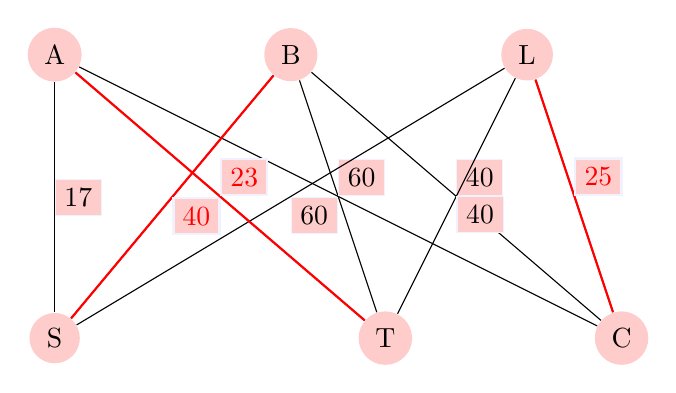
\begin{tikzpicture}
  [scale=.6,auto=left,every node/.style={circle,fill=red!20}]
  \tikzstyle{weight} = [draw=blue!5,shape=rectangle]
  \node (n1) at (-1,5) {A};
  \node (n2) at (4,5)  {B};
  \node (n3) at (9,5)  {L};
  \node (n4) at (-1,-1) {S};
  \node (n5) at (6, -1) {T};
  \node (n6) at (11,-1)  {C};
 
\foreach \source /\dest /\weight in {n1/n4/17,n1/n5/40,n1/n6/45} 
   \draw (\source) --node[weight] {$\weight$}  (\dest);
\foreach \source /\dest /\weight in {n2/n4/23,n2/n5/60,n2/n6/40} 
   \draw (\source) --node[weight] {$\weight$}  (\dest);
\foreach \source /\dest /\weight in {n3/n4/60,n3/n5/40,n3/n6/25} 
   \draw (\source) --node[weight] {$\weight$}  (\dest);
\foreach \source /\dest /\weight in {n2/n4/40,n1/n5/23,n3/n6/25} 
   \draw[color=red,thick] (\source) --node[weight] {$\weight$}  (\dest); 
 
  \end{tikzpicture}
\caption{Complete Bipartite Graph for Table \ref{16t3} - Notations: A is Al, B is Bob, L is Caleb, S is Salesman, T is Tutor and C is Chef. Weights represent the costs.Minimum Perfect matching edges are colored red.}\label{16g3}
\end{center}
\end{figure}

Ajur was more interested in why and how these procedures work. Rishnak said that he himself had not understood some of these things very well and that Ajur would learn it in college. This seemed to be all right to Ajur and he nodded and left with for a stroll. Rishnak was unhappy with himself that he did not study these things well enough to be able to explain to Ajur! 

